%\documentclass[11pt,fleqn,twoside]{article}
\documentclass{llncs}

\usepackage[english]{babel}
\usepackage{alltt}
\usepackage{graphicx}
\usepackage{url}
\usepackage{subfigure}
\usepackage{listings}
\usepackage{color}
\usepackage{lscape}
\usepackage{xspace}
\usepackage{latexsym}
\usepackage{rotating} 
\usepackage{enumitem}
\usepackage{verbatim}
\usepackage{url}
\usepackage{multirow}
\usepackage{chngcntr}

\begin{document}

\title{Notes on Physical \& Logical Data Layouts}
	\author{
	Michael Hausenblas\inst{1} 
	}
	\institute{MapR Technologies EMEA, Ireland\\
	\email{mhausenblas@maprtech.com}
	}
\maketitle

\begin{abstract}
In this short note I review and discuss fundamental options for physical and
logical data layouts as well as implications on data processing at large scales.
I should say in advance that these notes offer no new insights, that is, 
everything stated here has already been published elsewhere. In fact, it has
been published in so many different places, such as blog posts, in the 
literature, etc. that the main contribution is to bring it all together in one
place.
\end{abstract}

\section{Motivation}
\label{sec:mot}
Data processing and management systems such as databases, datastores or query 
engines usually have to answer to two kinds of entities: \emph{humans} and 
\emph{hardware}. 
Towards humans, they provide means to query, manipulate or 
manage\footnote{The management aspect can span a wide range of activities 
including but not limited to snapshots, mirroring, etc.} data.
Towards the hardware, they issue store and retrieve commands. They depend 
directly or indirectly on the very nature of the hardware. Almost all systems---
for example, Hadoop's distributed file system---are designed with strong though
not necessarily explicit assumptions about the underlying hardware such as hard 
disk drives\footnote{More at \url{http://queue.acm.org/detail.cfm?id=1317403}}, 
their spindles, heads, etc.

Conceptually, there are three levels present in data management systems
(Fig.~\ref{fig:data-layers}):
\begin{figure}[h!]
\centering
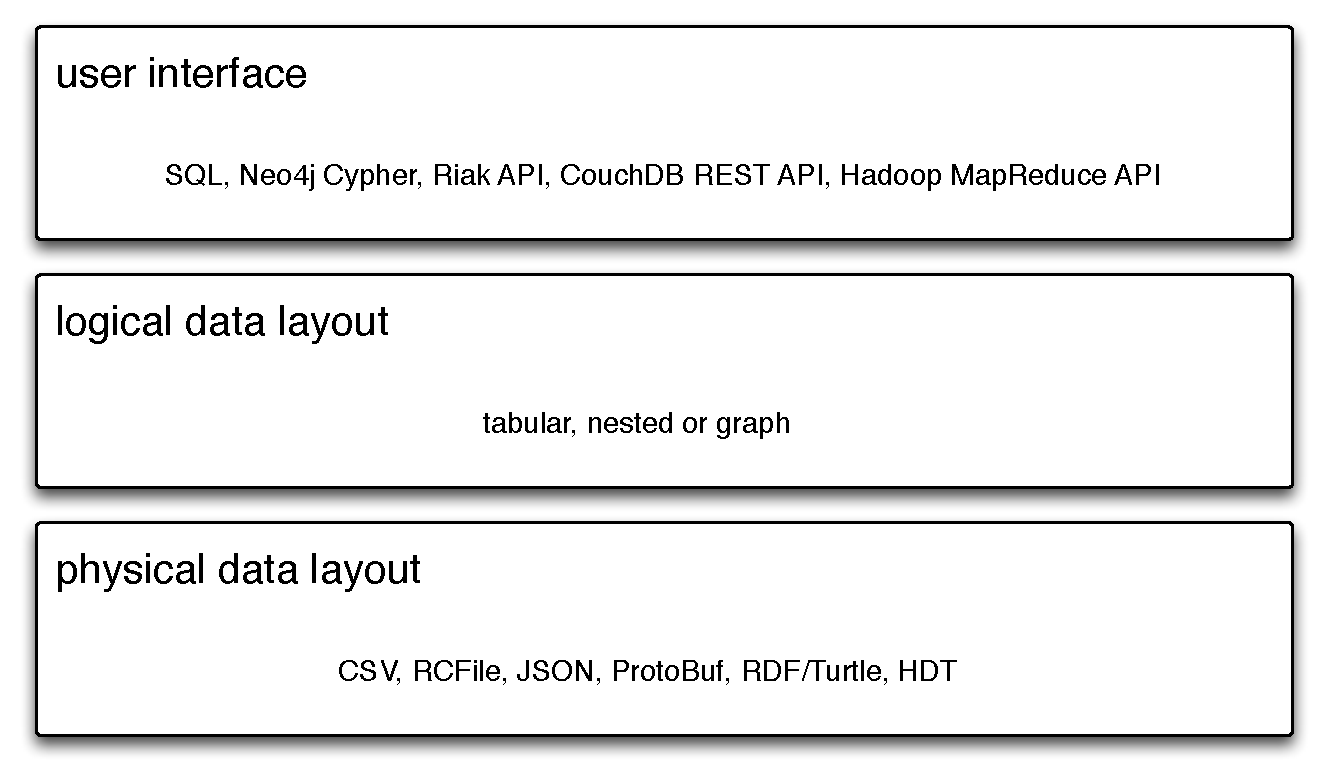
\includegraphics[width=0.7\textwidth]{data-layers}
\caption{The three levels of data representation and interaction in data 
management systems, including examples for each of the levels.}
\label{fig:data-layers}
\end{figure}
\begin{itemize}
\item The \emph{User Interface} level. Any database or datastore needs 
to provide a way to interact with the data under management. This can be 
something elaborate, standardised and mature as the Structured Query Language 
(SQL) found in relational database management systems (RDBMS), such as 
Oracle DB, PostgreSQL, or MySQL. This can be a RESTful interface, found in many 
NoSQL datastores, like, for example, CouchDB's API\footnote{See documentation at
\url{http://wiki.apache.org/couchdb/HTTP_Document_API}}. Of course, this can 
also be a programming-language-level API such as the case with
Hadoop\footnote{\url{http://hadoop.apache.org/docs/current/api/org/apache/hadoop
/mapreduce/package-summary.html}}.
\item The \emph{Logical Data Layout} level.
\item The \emph{Physical Data Layout} level.
\end{itemize}

\section{Manifestations of Data Layouts}
\label{sec:mani}
In~\cite{Hausenblas:arxiv2012} we introduced the three fundamental data shapes
\emph{tabular}, \emph{tree} or henceforth \emph{nested}, and \emph{graph}.


\begin{figure}[h!]
\centering
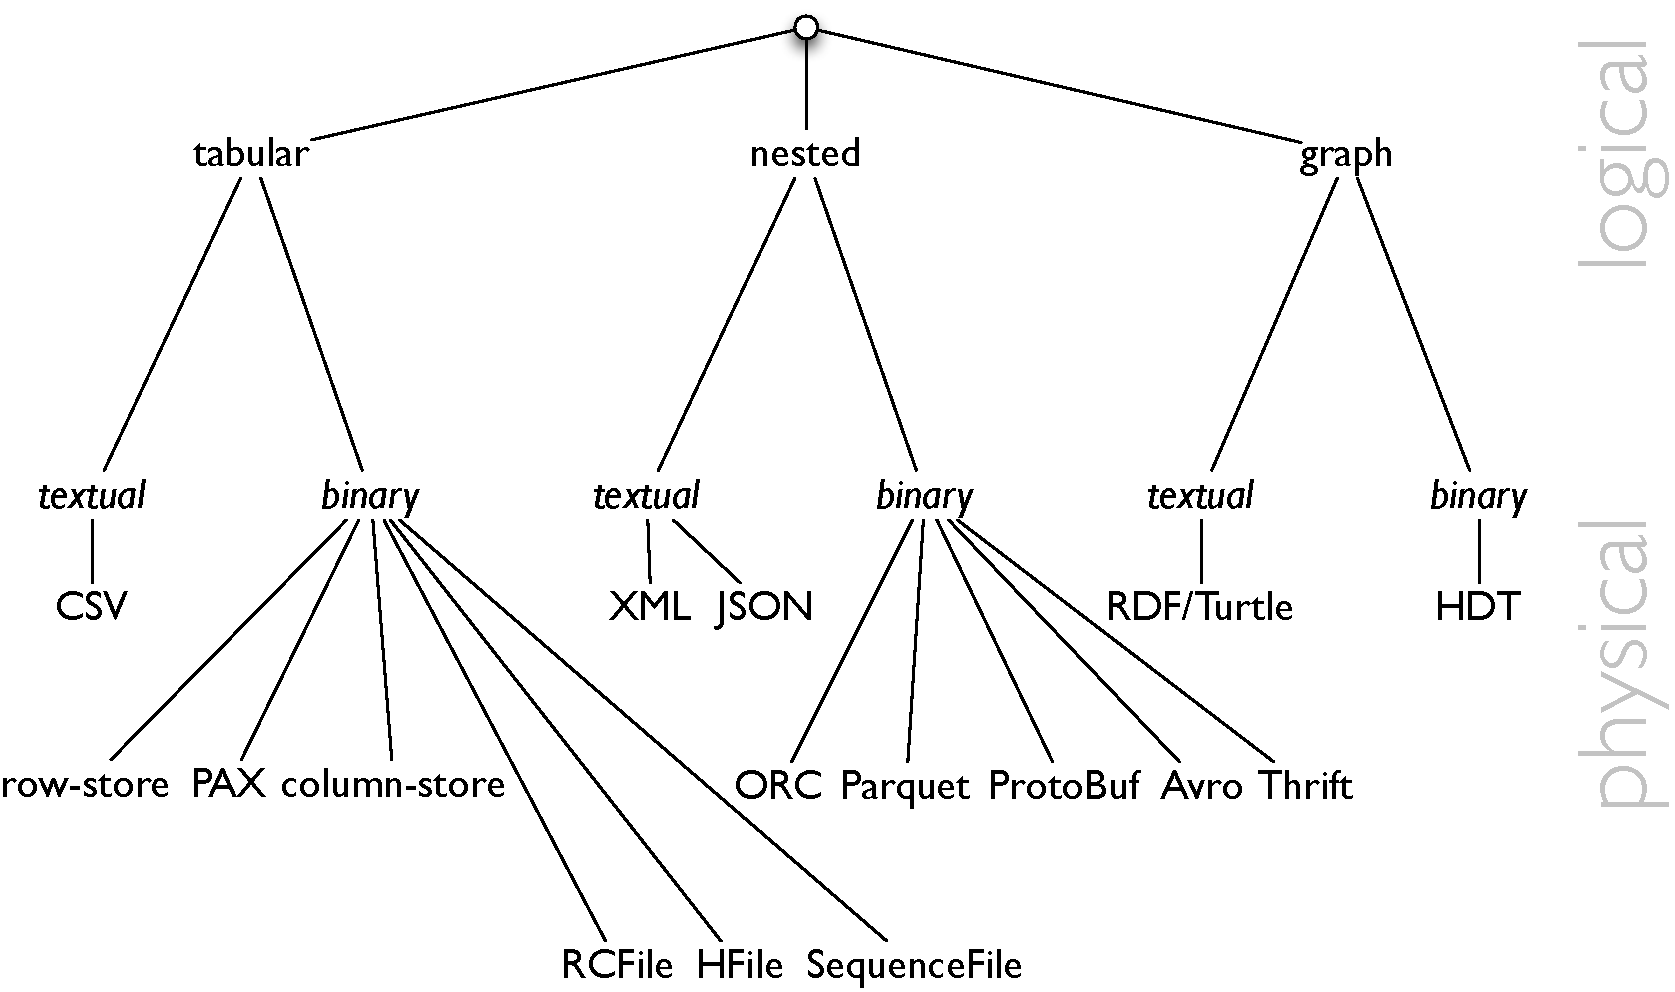
\includegraphics[width=0.9\textwidth]{taxonomy-dl}
\caption{A non-exhaustive, lightweight taxonomy for logical and physical data 
layouts and serialisation formats commonly used in the data processing 
community.}
\label{fig:taxonomy-dl}
\end{figure}


Normalised:
\begin{itemize}
	\item No need to handle duplicates on update.
	\item Built-in data integrity.
	\item Storage efficient (takes less disk space).
\end{itemize}

Denormalised:
\begin{itemize}
	\item Data access is fast.
	\item Provides entity-centric view.
	\item No joins necessary (pre-joined).
\end{itemize}

Summarised in Table~\ref{tab:ndcomparison}.

\begin{center}
\begin{table}
\caption{A comparison of normalised vs. denormalised handling of data on the 
logical and physical level across SQL and NoSQL data management systems.}
\label{tab:ndcomparison}
\begin{tabular}{l @{\hskip 2mm} p{0.40\linewidth} @{\hskip 5mm}
	            p{0.40\linewidth} @{\hskip 2mm}}
& \textbf{NORMALISED}& \textbf{DENORMALISED}\\
\hline
\hline
\emph{characteristics}&
Each data item is stored exactly in one place.&
The data items are repeated as needed.\\
\hline
\emph{advantages}&
Built-in data integrity and storage-efficiency.&
Fast, entity-centric data access without the need for joins.\\
\hline
\emph{disadvantages} &
Joints are costly and hard to implement (esp. distributed).&
Inflexible and storage-hungry.\\
\hline
\emph{workloads} &
OLTP, write-intensive&
OLAP, read-intensive\\
\hline
\emph{examples} &
Classical, textbook relational database modelling&
Wide-column datastores (HBase, Cassandra), document-oriented 
datastores (MongoDB, CouchDB), key-value datastores (Redis, Memcached, etc.),
graph databases (Neo4j, RDF stores), large-scale relational databases\\
\hline
\hline
\end{tabular}
\centering
\end{table}
\end{center}


\section{Impact on Data Processing at Scale}
\label{sec:ldp}


\section{Conclusions and Challenges}
\label{sec:concl}

\section{Acknowledgements}
\label{sec:ack}
I'd like to thank Eric Brewer, whose RICON2012 keynote motivated me to write up
this short note. His keynote is available via \url{https://vimeo.com/52446728} 
and more than certainly worth it watching it.

\bibliographystyle{alpha}
\bibliography{data-proc}


\end{document}

